% Options for packages loaded elsewhere
\PassOptionsToPackage{unicode}{hyperref}
\PassOptionsToPackage{hyphens}{url}
%
\documentclass[
]{book}
\usepackage{amsmath,amssymb}
\usepackage{iftex}
\ifPDFTeX
  \usepackage[T1]{fontenc}
  \usepackage[utf8]{inputenc}
  \usepackage{textcomp} % provide euro and other symbols
\else % if luatex or xetex
  \usepackage{unicode-math} % this also loads fontspec
  \defaultfontfeatures{Scale=MatchLowercase}
  \defaultfontfeatures[\rmfamily]{Ligatures=TeX,Scale=1}
\fi
\usepackage{lmodern}
\ifPDFTeX\else
  % xetex/luatex font selection
\fi
% Use upquote if available, for straight quotes in verbatim environments
\IfFileExists{upquote.sty}{\usepackage{upquote}}{}
\IfFileExists{microtype.sty}{% use microtype if available
  \usepackage[]{microtype}
  \UseMicrotypeSet[protrusion]{basicmath} % disable protrusion for tt fonts
}{}
\makeatletter
\@ifundefined{KOMAClassName}{% if non-KOMA class
  \IfFileExists{parskip.sty}{%
    \usepackage{parskip}
  }{% else
    \setlength{\parindent}{0pt}
    \setlength{\parskip}{6pt plus 2pt minus 1pt}}
}{% if KOMA class
  \KOMAoptions{parskip=half}}
\makeatother
\usepackage{xcolor}
\usepackage{longtable,booktabs,array}
\usepackage{calc} % for calculating minipage widths
% Correct order of tables after \paragraph or \subparagraph
\usepackage{etoolbox}
\makeatletter
\patchcmd\longtable{\par}{\if@noskipsec\mbox{}\fi\par}{}{}
\makeatother
% Allow footnotes in longtable head/foot
\IfFileExists{footnotehyper.sty}{\usepackage{footnotehyper}}{\usepackage{footnote}}
\makesavenoteenv{longtable}
\usepackage{graphicx}
\makeatletter
\newsavebox\pandoc@box
\newcommand*\pandocbounded[1]{% scales image to fit in text height/width
  \sbox\pandoc@box{#1}%
  \Gscale@div\@tempa{\textheight}{\dimexpr\ht\pandoc@box+\dp\pandoc@box\relax}%
  \Gscale@div\@tempb{\linewidth}{\wd\pandoc@box}%
  \ifdim\@tempb\p@<\@tempa\p@\let\@tempa\@tempb\fi% select the smaller of both
  \ifdim\@tempa\p@<\p@\scalebox{\@tempa}{\usebox\pandoc@box}%
  \else\usebox{\pandoc@box}%
  \fi%
}
% Set default figure placement to htbp
\def\fps@figure{htbp}
\makeatother
\setlength{\emergencystretch}{3em} % prevent overfull lines
\providecommand{\tightlist}{%
  \setlength{\itemsep}{0pt}\setlength{\parskip}{0pt}}
\setcounter{secnumdepth}{5}
% definitions for citeproc citations
\NewDocumentCommand\citeproctext{}{}
\NewDocumentCommand\citeproc{mm}{%
  \begingroup\def\citeproctext{#2}\cite{#1}\endgroup}
\makeatletter
 % allow citations to break across lines
 \let\@cite@ofmt\@firstofone
 % avoid brackets around text for \cite:
 \def\@biblabel#1{}
 \def\@cite#1#2{{#1\if@tempswa , #2\fi}}
\makeatother
\newlength{\cslhangindent}
\setlength{\cslhangindent}{1.5em}
\newlength{\csllabelwidth}
\setlength{\csllabelwidth}{3em}
\newenvironment{CSLReferences}[2] % #1 hanging-indent, #2 entry-spacing
 {\begin{list}{}{%
  \setlength{\itemindent}{0pt}
  \setlength{\leftmargin}{0pt}
  \setlength{\parsep}{0pt}
  % turn on hanging indent if param 1 is 1
  \ifodd #1
   \setlength{\leftmargin}{\cslhangindent}
   \setlength{\itemindent}{-1\cslhangindent}
  \fi
  % set entry spacing
  \setlength{\itemsep}{#2\baselineskip}}}
 {\end{list}}
\usepackage{calc}
\newcommand{\CSLBlock}[1]{\hfill\break\parbox[t]{\linewidth}{\strut\ignorespaces#1\strut}}
\newcommand{\CSLLeftMargin}[1]{\parbox[t]{\csllabelwidth}{\strut#1\strut}}
\newcommand{\CSLRightInline}[1]{\parbox[t]{\linewidth - \csllabelwidth}{\strut#1\strut}}
\newcommand{\CSLIndent}[1]{\hspace{\cslhangindent}#1}
\usepackage{booktabs}
\usepackage{bookmark}
\IfFileExists{xurl.sty}{\usepackage{xurl}}{} % add URL line breaks if available
\urlstyle{same}
\hypersetup{
  pdftitle={Medida e Integração (Segunda Edição)},
  pdfauthor={Pedro J. Fernandez},
  hidelinks,
  pdfcreator={LaTeX via pandoc}}

\title{Medida e Integração (Segunda Edição)}
\author{Pedro J. Fernandez}
\date{1976}

\begin{document}
\maketitle

{
\setcounter{tocdepth}{1}
\tableofcontents
}
\chapter*{Prefácio}\label{prefuxe1cio}
\addcontentsline{toc}{chapter}{Prefácio}

O presente livro vem tentar preencher a necessidade cada vez mais imperiosa de proporcionar, num programa de Mestrado em Matemática ou Estatística Matemática, uma versão da Teoria da Medida que permita ``uma aplicação mais ou menos imediata a outras áreas, como por exemplo Teoria ``das Probabilidades, Estatística Matemática e suas ramificações, Física Matemática, etc.

Com esse objetivo em mente, apresentamos uma versão abstrata da Teoria da Medida com abundantes referências ao caso da medida de Lebesgue em \(\mathbb{R}^n\) e outros exemplos importantes. Creio que, com o mesmo esforço e muito menos tempo, é possível estudar e compreender direta- mente uma versão abstrata da Teoria da Medida não passando pelo estudo da medida de Lebesgue em \(\mathbb{R}^1\) ou \(\mathbb{R}^n\), Porém se recomenda fortemente ao leitor, interpretar, sempre que possível, cada definição ou resultado em termos da medida de Lebesgue em \(\mathbb{R}^1\) ou \(\mathbb{R}^n\), Este é o exemplo que em ``primeira aproximação'' deve dominar a mente do leitor. O leitor é também fortemente encorajado a consultar outras obras de Teoria da Medida como as citadas em \citeproc{ref-1}{{[}1{]}}, \citeproc{ref-2}{{[}2{]}}, \citeproc{ref-3}{{[}3{]}}, \citeproc{ref-4}{{[}4{]}}, \citeproc{ref-5}{{[}5{]}}, \citeproc{ref-6}{{[}6{]}} e \citeproc{ref-9}{{[}7{]}}, das Referências.

Como acontece frequentemente em todas as ciências, a aplicação de uma teoria em outra área do conhecimento produz um ``feedback''. No caso particular da utilização da Teoria da Medida para formalizar as noções básicas de Probabilidades, a resposta foi tremenda. A quantidade de novos problemas e técnicas introduzidas superou rapidamente em volume a Teoria original. Não é objetivo desta obra entrar em Teoria das Probabilidades, mas o leitor que queira desfrutar da utilização das técnicas desenvolvidas neste livro numa apaixonante aplicação, é aconselhado a fazer um curso nessa disciplina ao nível de, por exemplo \citeproc{ref-13}{{[}8{]}}, \citeproc{ref-14}{{[}9{]}} ou \citeproc{ref-15}{{[}10{]}}. Este livro está preparado para que se entre diretamente no assunto, evitando perda de tempo com transições nem sempre bem sucedidas.

O material deste livro foi testado em diversas oportunidades no curso de Integração do IMPA. Em quatro dessas ocasiões o manuscrito foi lido cuidadosamente pelos Professores Manfredo Perdigão do Carmo, Jaime Lesmes e Carlos Isnard do IMPA, e pelo Professor Ernst Eberlein agora na Universidade de Bonn. Suas observações e comentários foram incorporados nesta obra, A eles, meu agradecimento muito especial. Desejo agradecer também a todos os alunos que participaram desses cursos (especialmente ao Flávio C. Bartmann) e que colaboraram indiretamente, através de perguntas, sugestões e dúvidas, para dar forma final a esta obra. Desejo finalmente agradecer a todos os meus colegas do IMPA por proporcionar, como sempre, o incentivo e o ambiente de camaradagem e dedicação permanente ao trabalho científico, tão necessários para escrever obras como esta.

Rio de Janeiro, março de 1976

Pedro J. Fernandez

\chapter*{Introdução}\label{introduuxe7uxe3o}
\addcontentsline{toc}{chapter}{Introdução}

Para a leitura deste livro é essencial que o leitor tenha realizado anteriormente um curso de Cálculo Diferencial em várias variáveis reais e outro de Funções Reais. Seria conveniente que conhecesse os temas mais importantes de um curso de Análise no \(\mathbb{R}^n\), noções gerais de espaços topológicos, e algumas definições e propriedades básicas de Espaços de Banach. Porém o requisito talvez mais importante é o de ter um pouco de maturidade matemática. Por essa razão é aconselhável que um curso baseado neste livro seja deixado para a segunda metade de um programa de mestrado. A notação usada é a usual em outros livros e textos gerais de matemática. Alguns símbolos que achamos que não sejam frequentemente usados, são indicados a seguir.

O supremo e ínfimo de dois números reais \(a\) e \(b\), serão indicados por \(a \lor b\) e \(a \land b\) , respectivamente verifica-se facilmente que: \[a \lor b = \frac{1}{2}(a + b + |a - b|)\] e \[a \land b = \frac{1}{2}(a + b - |a - b|)\] Se \(a\) e \(b\) são números reais, teremos sempre: \[|a+b| \le |a| + |b| \quad \text{e} \quad ||a|-|b|| \le |a-b|.\]

Se \(f\) e \(g\) são funções reais, definimos a função máximo (supremo) de \(f\) e \(g\) (\(f \lor g\)) e mínimo (ínfimo) de \(f\) e \(g\) (\(f \land g\)) pelas fórmulas: \[(f \lor g)(x) = f(x) \lor g(x) \quad \text{e} \quad (f \land g)(x) = f(x) \land g(x).\] Caso \(g=0\), escrevemos \(f^{+}\) em lugar de \(f \lor 0\), e \(f^{-}\) em lugar de \(-(f \land 0)\). Resulta então que, \(|f| = f^{+} + f^{-}\), e \(f = f^{+} - f^{-}\).

Se \(\{x_n\}_{n=1,2,...}\) é uma sucessão de números reais, definimos o limite superior e o limite inferior de tal sucessão, de acordo com as fórmulas: \[ \lim_n \sup x_n = \inf_n \sup \{x_k : k \ge n\}, \] \[ \lim_n \inf x_n = \sup_n \inf \{x_k : k \ge n\}. \] Temos que \(-\infty \le \lim_n \inf x_n \le \lim_n \sup x_n \le +\infty\).

Por outro lado, sendo \(\{f_n\}_{n=1,2,...}\) uma sucessão de funções, podemos naturalmente definir \(\lim_n \sup f_n\) e \(\lim_n \inf f_n\) como as funções: \[\begin{gathered} (\lim_n \sup f_n)(x) = \lim_n \sup f_n(x). \\ (\lim_n \inf f_n)(x) = \lim_n \inf f_n(x). \end{gathered} \]

Se uma série converge de modo absoluto (\emph{série absolutamente convergente}), será por vezes indicada com a notação \(\sum\limits_{n=1}^{\infty} |x_n| < \infty\).

Se \(\{x_n\}_{n=1,2,...}\) converge a \(x\) escreveremos \(x_n \to x\). Se \(\{x_n\}_{n=1,2,...}\) é crescente (decrescente) e converge a \(x\) escreveremos \(x_n \uparrow x\) \((x_n \downarrow x)\). O maior inteiro menor ou igual ao número real \(x\) será denotado por \([x]\) (parte inteira de \(x\)). A menos de mencionado o contrário a letra \(\mathbb{N}\) indicará o conjunto \(\mathbb{N} = \{1, 2, ...\}\). \(\mathbb{R}^1\) denotará o conjunto dos números reais e \(\mathbb{R}^n = \mathbb{R}^1 \times \mathbb{R}^1 \times \dots \times \mathbb{R}^1\) o produto cartesiano de \(\mathbb{R}^1\) \(n\) vezes.

Vamos agora fazer uma descrição geral do conteúdo, motivações e objetivos desta obra.

No Cap. 0 o leitor vai encontrar uma revisão rápida das noções básicas da Teoria dos Conjuntos. O propósito do capítulo é relembrar ao leitor certas propriedades, definições e teoremas básicos, e fundamentalmente fixar uma notação que será utilizada constantemente nos capítulos seguintes. A obra de P. R. Halmos mencionada na referência {[}16{]} pode ser consultada para maiores detalhes.

Consideremos, para fixar as ideias, a família de retângulos no plano real \(\mathbb{R}^2\). \[ S = \{D_1 \times D_2: D_i \text{ é intervalo de } \mathbb{R}^1, i=1, 2\} \] Por intervalo entendemos qualquer intervalo finito, aberto, fechado ou semi-aberto de \(\mathbb{R}^1\).

Definimos sobre \(S\) a seguinte função de conjunto: \[ \lambda(D_1 \times D_2) = (b_1 - a_1)(b_2 - a_2) \] onde \(a_1 \le b_1\) são os extremos de \(D_1\) e \(a_2 \le b_2\) são os extremos de \(D_2\). \(\lambda\) é a medida (a área) de \(D_1 \times D_2\).

Um dos problemas básicos da Teoria da Medida é a de ``aumentar'' (estender) a classe dos conjuntos que sejamos capazes de medir (para os quais possamos definir um número que será a sua área) de forma tal que a área de um retângulo seja o produto dos comprimentos dos lados e de maneira que essa medida tenha propriedades ``razoáveis'' e matematicamente interessantes.

Como acontece freqüentemente em matemática depois de um certo tempo, foram isoladas às propriedades possuídas pela classe dos retângulos e a função de conjunto-área, que tornavam possível uma extensão.

A classe dos retângulos tem exatamente as propriedades que definem um semi-anel (Definição 1.1) e a função \(\lambda\) satisfaz as condições

\begin{enumerate}
\def\labelenumi{\roman{enumi})}
\item
  \(\lambda(\varnothing) = 0, \lambda \ge 0\)
\item
  \(\lambda\left(\sum\limits_{i=1}^\infty C_i\right) = \sum\limits_{i=1}^\infty \lambda(C_i)\) se \(C_i; i=1, 2, \dots\) e \(\sum\limits_{i=1}^\infty C_i\) pertencem a \(\mathbb{S}\).
\end{enumerate}

Uma função de conjunto com as propriedades i) e ii) é chamada de medida (neste caso uma medida sobre um semi-anel).

O problema então pode ser formulado da seguinte maneira. Dado um semi-anel \(\mathbb{S}\) de subconjuntos de um conjunto fixo \(\Omega\) e uma medida \(\mu\) sobre um semi-anel, \emph{estender} esta função a uma classe de conjuntos \(\Lambda\), a maior possível, de maneira tal que essa extensão conserve as propriedades i) e ii) que definem uma medida.

O resultado mais importante é o seguinte:

\textbf{Teorema} (Teorema de extensão) Dada uma medida \(\mu\) sobre um semi-anel \(\mathbb{S}\), existem um \(\sigma\)-anel \(\Lambda, \Lambda \supseteq \mathbb{S}\), e uma medida completa \(\mu\) sobre \(\Lambda\) que é uma extensão de \(\mu\). Se \(\mu\) é \(\sigma\)-finita sobre \(\mathbb{S}\) então a extensão é única.
:::

O Cap. 1 estuda diferentes classes de conjuntos sobre as quais as funções de conjunto introduzidas no Cap. 2 vão ser definidas. O teorema enunciado acima está contido no Cap. 2 e é obtido depois de uma série de resultados técnicos muitos deles com interesse independente. O procedimento de extensão é trabalhoso e vai requerer do leitor atenção, concentração e força de vontade para ler os detalhes até o fim. Na minha opinião vale a pena fazer o esforço logo no início pela familiaridade que se obtém na manipulação de conjuntos mensuráveis, facilitando dessa forma a leitura dos capítulos seguintes.

Estando já de posse da noção de espaço de medida e de numerosos exemplos construídos e estudados no Cap. 2, o Cap. 3 passa a estudar funções reais definidas nestes espaços. Seja \((\Omega, \mathscr{A}, \mu)\) um espaço de medida e \(f\) uma \emph{função simples}, i. e. \(f = \sum_{i=1}^{n} a_i I_{A_i}\) onde \(A_i \in \mathscr{A}\) e \(a_i \in \mathbb{R}^1\). Em outras palavras \(f\) toma um número finito de valores cada um deles sobre um conjunto mensurável (veja a figura seguinte).

Para uma função simples é natural definir a sua integral (área abaixo da função) como

\begin{center}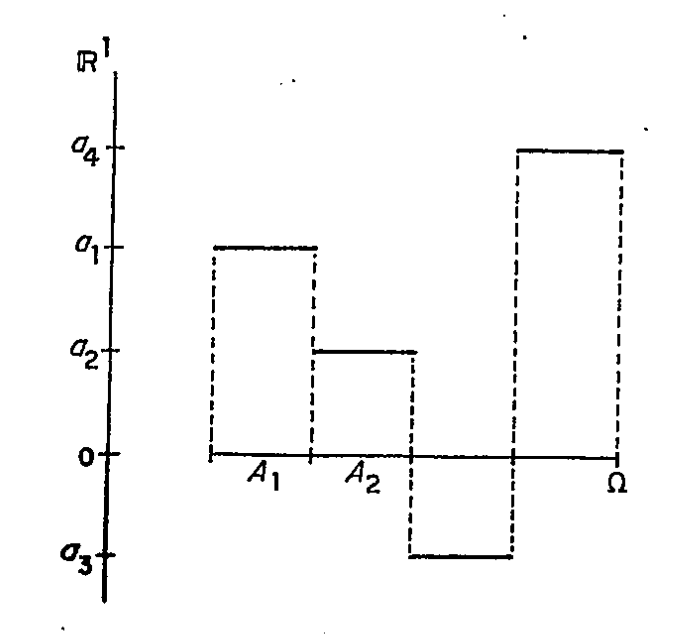
\includegraphics[width=9.49in]{figures/figure-00-01-01} \end{center}

\[ \int_{\Omega} f d\mu = \sum_{i=1}^{n} a_i \mu(A_i). \]

Seja \(f\) uma função real definida sobre \(\Omega\). Se \(f\) tem a seguinte propriedade: \(\forall a, b\) reais \(a \le b, \quad f^{-1}((a, b)) \in \mathscr{A}\), então \(f\) é um limite pontual de funções simples e reciprocamente. Para estas funções (chamadas funções mensuráveis) é natural definir a sua integral como o limite das integrais de uma seqüência de funções simples que convergem a ela. Ou seja, se \(g\) é uma função mensurável e \(f_n \to g\) onde \(\forall n, f_n\) é uma função simples, definimos: \[ \int g d\mu = \lim_{n} \int f_n d\mu. \] A menos de detalhes técnicos esta definição funciona e proporciona uma integral para a qual a fórmula \[ \int_{\Omega} (\lim_n f_n) d\mu = \lim_n \int_{\Omega} f_n d\mu \] que intercambia integral e limite é válida sob certas condições de regularidade não muito restritivas {[}Teorema 4.1.1 (Fatou-Lebesgue){]}.* O Cap. 4 é concluído com diversas aplicações da Integral de Lebesgue e com um estudo de dualidade entre espaços \(L_p\), estes últimos importante exemplo de espaços de Banach.

*Resulta também que toda função integrável Riemann é integrável Lebesgue, e as integrais coincidem.

No Cap. 5 é estudado o problema da construção de um espaço de medida utilizando outros espaços de medida (espaços-fatores). Consideremos para fixar idéias que temos dois espaços de medida \((\Omega_1, \mathscr{A}_1, \mu_1)\) e \((\Omega_2, \mathscr{A}_2, \mu_2)\). Sobre o conjunto produto \(\Omega = \Omega_1 \times \Omega_2\), seja \(\mathscr{A}\) a \(\sigma\)-álgebra gerada pelos conjuntos da forma \(A_1 \times A_2\) onde \(A_1 \in \mathscr{A}_1\) e \(A_2 \in \mathscr{A}_2\) (esta \(\sigma\)-álgebra é chamada \(\sigma\)-álgebra-produto). Sob certas condições de regularidade é provada a existência de uma única medida \(\nu\) sobre \(\mathscr{A}\) tal que: \[ \forall A_1 \in \mathscr{A}_1, \forall A_2 \in \mathscr{A}_2, \quad \nu(A_1 \times A_2) = \mu_1(A_1) \times \mu_2(A_2), \] \(\nu\) é chamada medida-produto.

Se \(f\) é uma função \(\mathscr{A}\)-mensurável e \(\nu\)-integrável, a seguinte fórmula é válida: \[ \begin{aligned} \int_{\Omega} f d\nu &= \int_{\Omega_1} \left[ \int_{\Omega_2} f(\omega_1, \omega_2) \mu_2(d\omega_2) \right] \mu_1(d\omega_1) \\ &= \int_{\Omega_2} \left[ \int_{\Omega_1} f(\omega_1, \omega_2) \mu_1(d\omega_1) \right] \mu_2(d\omega_2), \end{aligned} \] ou seja, a integral dupla coincide com as integrais iteradas (Teoremas de Tonelli e Fubini).

O Cap. 5 finaliza apresentando os produtos de um número infinito de espaços de medida, básicos na Teoria das Probabilidades e na modelagem de experimentos estatísticos.

Estuda-se no Cap. 6 as medidas que podem tomar valores positivos e negativos (medidas com sinal). Um exemplo importante é obtido da seguinte forma. Seja \((\Omega, \mathscr{A}, \mu)\) um espaço de medida e \(f\) uma função integrável com relação a \(\mu\). A função de conjunto: \[ \nu(A) = \int_{A} f d\mu, \quad A \in \mathscr{A} \] é uma medida com sinal.

Note que neste exemplo ``\(\nu\) é pequena se \(\mu\) é pequena''. Basicamente esta condição é suficiente para que \(\nu(A)\) seja obtida integrando uma função fixa \(f\) com relação a \(\mu\) sobre o conjunto \(A\). (Teorema de Radon-Nikodym).

Outro resultado muito importante contido no Cap. 6, é o que estabelece que toda medida com sinal é a diferença de duas medidas positivas (Decomposição de Jordan).

No Cap. 7 são estudadas as relações entre derivação e integração: em que sentido e sob quais condições derivar e integrar são operações inversas?

Seja \(f\) uma função definida em \(\mathbb{R}^1\) e integrável Lebesgue. Quando \[ \frac{d}{dx} \int_{a}^{x} f(y) dy = f(x)? \] Se \(x\) é um ponto de continuidade de \(f\), é bem conhecido pela teoria de integral de Riemann, que a igualdade é válida. Vai ser provado neste capítulo um resultado muito mais profundo: o de que a igualdade é válida em quase todo ponto. (Teorema de Diferenciação de Lebesgue).

Outra pergunta natural e importante é a seguinte: quando \[ \int_{a}^{b} f'(y) dy = f(b) - f(a)? \] Nesse capítulo vamos caracterizar a classe das funções para as quais esta igualdade é válida (funções absolutamente contínuas).

Não é possível, usando a integral de Lebesgue, reconstruir uma função conhecendo a sua derivada. Dá-se exemplos de funções com derivada finita em todo ponto de um intervalo mas não integráveis. Se a derivada é integrável e finita temos um resultado positivo: o Teor. 7.5.1 prova que a função é integral indefinida de sua derivada.

O capítulo contém vários resultados clássicos muito importantes como o \emph{Teorema de Lebesgue} sobre diferenciação de funções monótonas (toda função monótona é derivável em quase todo ponto) e um teorema sobre mudança de variáveis na Integral de Lebesgue.

Diversas funções que devem figurar na bagagem de todo matemático são construídas. Por exemplo, uma função contínua, estritamente crescente e com derivada nula em quase todo ponto.

\chapter{Conjuntos}\label{conjuntos}

\section{Conjuntos}\label{conjuntos-1}

Neste livro, toda vez que usamos a palavra conjunto queremos significar um subconjunto de um conjunto fixo, que em geral designaremos por \(\Omega\).

\(\Omega\) é chamado espaço, e seus elementos, pontos.
Se \(A\) é um subconjunto de \(\Omega\), a notação \(\omega \in A\) significa que \(\omega\) é um elemento de \(A\).
O fato de \(\omega\) não pertencer a \(A\) será indicado com a notação \(\omega \notin A\).
Se \(A\) e \(B\) são subconjuntos de \(\Omega\), a notação \(A \subseteq B\) indicará que todo elemento de \(A\) também pertence a \(B\).
A notação \(A \subset B\) indicará que \(A \subseteq B\), porém existe algum ponto de \(B\) que não é elemento de \(A\).

Com o objetivo de facilitar a notação, usaremos um conjunto que não contenha nenhum elemento, ao qual chamaremos conjunto vazio, e denotaremos por \(\varnothing\).

Usaremos as palavras classe ou família, para um conjunto de conjuntos.
A classe de todos os subconjuntos de um conjunto \(A\) será indicada por \(\mathbb{P}(A)\) (partes de \(A\)).

Para indicar um conjunto, também usaremos a notação \(\{\omega: p(\omega)\}\), onde \(p(\omega)\) é uma proposição concernente a \(\omega\), e o conjunto consiste de todos os elementos para os quais \(p(\omega)\) é verdadeira.
Por exemplo, \(\{\omega: \omega = 2k; k=1, 2, ...\}\) é o conjunto de todos os inteiros positivos pares.

Conjuntos finitos serão por vezes indicados pela designação de seus elementos.
Assim, o conjunto que consiste nos números 0, 2 e 4 será indicado \(\{0, 2, 4\}\).

É importante distinguir entre o ponto \(\omega\) e o conjunto \(\{\omega\}\), cujo único elemento é \(\omega\).

\section{Operações com conjuntos}\label{operauxe7uxf5es-com-conjuntos}

Seja \(\Gamma\) um certo conjunto de índices e, para cada \(\gamma \in \Gamma\), consideremos \(A_{\gamma}\), um subconjunto de \(\Omega\).
Chamaremos de união da família \(\{A_{\gamma}: \gamma \in \Gamma\}\) o conjunto de todos os pontos que pertencem a pelo menos um dos conjuntos \(A_{\gamma}\).
Esse conjunto será simbolizado por: \[ \bigcup_{\gamma \in \Gamma} A_{\gamma} = \{\omega: \exists \gamma \in \Gamma, \text{ tal que } \omega \in A_{\gamma}\}. \]

Se o conjunto \(\Gamma\) for enumerável, pode-se dizer que a família \(\{A_{\gamma}: \gamma \in \Gamma\}\) é uma sucessão \(\{A_n\}_{n=1,2,...}\).

Indicaremos, neste caso, a união por \(\bigcup\limits_{n=1}^{\infty} A_n\).

Se \(\Gamma = \{1, 2, ..., k\}\), a união será indicada por \(\bigcup\limits_{n=1}^{k} A_n\).

A união de dois conjuntos \(A\) e \(B\), será indicada por \(A \cup B\).

Se \(\Gamma = \varnothing\), \(\bigcup\limits_{\gamma \in \Gamma} A_{\gamma} = \varnothing\) por convenção.

Se \(\{A_{\gamma}: \gamma \in \Gamma\}\) é uma família de conjuntos, o conjunto de todos os elementos que pertencem a todos os \(A_{\gamma}\) será chamado interseção da família, e simbolizado por: \[ \bigcap_{\gamma \in \Gamma} A_{\gamma} = \{\omega: \forall \gamma, \omega \in A_{\gamma}\}. \]

Se \(\Gamma = \varnothing\), estabelecemos por convenção que \(\bigcap\limits_{\gamma \in \Gamma} A_{\gamma} = \Omega\).

Como no caso da união de conjuntos, conforme \(\Gamma\) seja enumerável, finito, ou conste de dois elementos, usaremos as notações: \[\bigcap\limits_{n=1}^{\infty} A_n, \bigcap\limits_{n=1}^{k} A_n, A \cap B.\]

Quando falarmos de interseção finita ficará subentendido que \(\Gamma \neq \varnothing\).

Dois conjuntos são ditos disjuntos, se \(A \cap B = \varnothing\).
Uma família \(\{A_{\gamma}: \gamma \in \Gamma\}\) se diz disjunta, se para todo par de elementos \(\gamma, \gamma' \in \Gamma\), com \(\gamma \neq \gamma'\), \(A_{\gamma} \cap A_{\gamma'} = \varnothing\).

Neste caso, usaremos a notação \(\sum\limits_{\gamma \in \Gamma} A_{\gamma}\), em lugar de \(\bigcup\limits_{\gamma \in \Gamma} A_{\gamma}\), para indicar a união da família.

Dado \(A \subseteq \Omega, A^c\) denotará o conjunto dos pontos que não pertencem a \(A\).
Em símbolos, \(A^c = \{\omega: \omega \notin A\}\).
\(A^c\) é chamado complemento de \(A\).

A diferença entre \(A\) e \(B\), simbolizada por \(A-B\), é, por definição, o conjunto \(A-B = A \cap B^c\).

Tal diferença será chamada própria, se \(B \subseteq A\).
Ao conjunto \((A-B) + (B-A)\), designado por \(A \Delta B\), chamaremos diferença simétrica entre \(A\) e \(B\).

Apresentamos, a seguir, uma série de importantes relações que serão usadas sem menções explícitas, nos capítulos seguintes.
Suas demonstrações são deixadas como exercícios.

\(\forall A, A \subseteq \Omega; A \cup \varnothing = A, A \cap \varnothing = \varnothing\).

\(A \subseteq B\) se, e somente se, \(A \cup B = B\).

\(A \cup (B \cup C) = (A \cup B) \cup C\).

\(A \cap (B \cap C) = (A \cap B) \cap C\).

\(A \cap (B \cup C) = (A \cap B) \cup (A \cap C)\).

\(A \cup (B \cap C) = (A \cup B) \cap (A \cup C)\).

\(A \cap (\bigcup\limits_{\gamma \in \Gamma} A_{\gamma}) = \bigcup\limits_{\gamma \in \Gamma} (A \cap A_{\gamma})\).

\(A \cup (\bigcap\limits_{\gamma \in \Gamma} A_{\gamma}) = \bigcap\limits_{\gamma \in \Gamma} (A \cup A_{\gamma})\).

\(A + A^c = \Omega, A \cap A^c = \varnothing, \Omega^c = \varnothing, \varnothing^c = \Omega\).

\((A^c)^c = A\); \(A \subseteq B\) se, e somente se, \(B^c \subseteq A^c\).

\((\bigcup\limits_{\gamma \in \Gamma} A_{\gamma})^c = \bigcap\limits_{\gamma \in \Gamma} (A_{\gamma}^c)\).

\((\bigcap\limits_{\gamma \in \Gamma} A_{\gamma})^c = \bigcup\limits_{\gamma \in \Gamma} (A_{\gamma}^c)\).

\(A \Delta B \subseteq (A \Delta C) \cup (B \Delta C), \forall C \subseteq \Omega\).

\section{Limites e indicadores}\label{limites-e-indicadores}

Se \(\{A_n\}_{n=1,2,...}\) é uma sucessão de conjuntos, chamaremos limite superior da sucessão \(\{A_n\}_{n=1,2,...}\) ao conjunto de todos os pontos \(\omega\) que pertençam a \(A_n\), para infinitos valores de \(n\).
É fácil ver que: \[ \lim_n \sup A_n = \bigcap_{n=1}^{\infty} \bigcup_{i=n}^{\infty} A_i. \]

O conjunto de todos os pontos de \(\Omega\) que pertencem a todos os \(A_n\), a menos de um número finito de tais \(A_n\), é chamado limite inferior da sucessão \(\{A_n\}_{n=1,2,...}\), e simbolizado por \(\lim_n \inf A_n\).
É fácil provar, de maneira análoga ao caso anterior, que: \[ \lim_n \inf A_n = \bigcup_{n=1}^{\infty} \bigcap_{i=n}^{\infty} A_i. \]

Uma sucessão \(\{A_n\}_{n=1,2,...}\) é dita crescente (respectivamente, decrescente), se \(A_n \subseteq A_{n+1}, n=1, 2, ...\) (resp. \(A_n \supseteq A_{n+1}, n=1, 2, ...\)).

Se para uma sucessão \(\{A_n\}_{n=1,2,...}\), \(\lim_n \sup A_n = \lim_n \inf A_n\), diremos que tal sucessão tem limite, e então empregaremos apenas a notação \(\lim_n A_n\).
Indicaremos sucessões crescentes (resp. decrescentes) de conjuntos com a notação \(A_n \uparrow\) (resp. \(A_n \downarrow\)).
Escreveremos \(A_n \uparrow A\) (resp. \(A_n \downarrow A\)) se \(A_n \uparrow\) (resp. \(A_n \downarrow\)), e \(\bigcup\limits_{n=1}^{\infty} A_n = A\) (resp. \(\bigcap\limits_{n=1}^{\infty} A_n = A\)).

Dado \(A \subseteq \Omega\), chamaremos indicador de \(A\), a função \(I_A\) definida por: \[ I_A(\omega) = \begin{cases} 1, & \omega \in A \\ 0, & \omega \notin A \end{cases}. \]

Existe claramente uma correspondência biunívoca (bijeção) entre subconjuntos de \(\Omega\) e seus indicadores correspondentes.
Esta noção nos será extremamente útil nos capítulos seguintes.
A seguir, apresentaremos algumas fórmulas, que são deixadas a título de exercício.
É importante que o leitor se familiarize com o manejo de indicadores.

\(A \subseteq B\) se, e somente se, \(I_A \le I_B, I_{A^c} = 1 - I_A\).

\(I_{A \cap B} = I_A \wedge I_B = I_A I_B\); \(I_{\bigcap\limits_{i=1}^n A_i} = \prod\limits_{i=1}^n I_{A_i}\).

\(I_{A \cup B} = I_A + I_B - I_A I_B = I_A \vee I_B\).

\(I_{(\bigcup\limits_{i=1}^n A_i)} = 1 - \prod\limits_{i=1}^n (1-I_{A_i}) = \sum\limits_{k=1}^n (-1)^{k-1} \sum\limits_{1 \le i_1 < i_2 < \dots < i_k \le n} \quad \prod\limits_{j=1}^k I_{A_{i_j}}\).

\(I_{(A \Delta B)} = I_A + I_B - 2 I_A I_B = |I_A - I_B|\).

\(I_{(A-B)} = I_A(1 - I_B)\).

\(I_{\lim_n \sup A_n} = \lim_n \sup I_{A_n}\); \(I_{\lim_n \inf A_n} = \lim_n \inf I_{A_n}\).

\section{Funções}\label{funuxe7uxf5es}

Sendo \(X\) e \(Y\) dois conjuntos, denotamos por \(Y^X\) o conjunto de todas as funções de \(X\) em \(Y\).

Se \(A \subseteq Y\) e \(f\) é uma função, usamos a notação \(f^{-1}(A)\), ou às vezes \([f \in A]\), para indicar o conjunto \(\{x: f(x) \in A\}\).
Se \(B \subseteq X\), \(f(B)\) representará o conjunto \(\{y: \exists x \in B: y = f(x)\}\).

Usaremos, sem menção explícita, as seguintes fórmulas facilmente verificáveis:

0.4.1.
\(f^{-1}(A^c) = [f^{-1}(A)]^c\); \(A \subseteq Y\).
0.4.2.
\(f^{-1}(\bigcap\limits_{\alpha \in I} A_{\alpha}) = \bigcap\limits_{\alpha \in I} f^{-1}(A_{\alpha})\), \(f^{-1}(\bigcup\limits_{\alpha \in I} A_{\alpha}) = \bigcup\limits_{\alpha \in I} f^{-1}(A_{\alpha})\), onde \(\{A_{\alpha}\}_{\alpha \in I}\) é uma família de subconjuntos de \(Y\).
0.4.3.
\(f(\bigcup\limits_{\alpha \in I} B_{\alpha}) = \bigcup\limits_{\alpha \in I} f(B_{\alpha})\), \(\{B_{\alpha}\}_{\alpha \in I}\) é uma família de subconjuntos de \(X\).
0.4.4.
\(f(\bigcap\limits_{\alpha \in I} A_{\alpha}) \subseteq \bigcap\limits_{\alpha \in I} f(A_{\alpha})\).

Se \(A \subseteq X\) e \(f: X \to Y\), a notação \(f|_A\) é a função pertinente a \(Y^A\), definida por:

\[f|_A(x) = f(x), \text{ onde chama-se } f|_A \text{ a restrição de } f \text{ a } A.\]

\section*{Exercícios}\label{exercuxedcios}
\addcontentsline{toc}{section}{Exercícios}

\begin{enumerate}
\def\labelenumi{\arabic{enumi}.}
\tightlist
\item
  Provar as fórmulas das Seqs. 0.2, 0.3 e 0.4.
\item
  Descrever por palavras o conjunto: \[ \lim_n \sup A_n - \lim_n \inf A_n. \]
\item
  Escrever a união e a diferença de dois conjuntos, utilizando as operações \(\Delta\) e \(\cap\).
\item
  Seja \(\{x_1, x_2, ...\}\) uma enumeração dos racionais de \(\mathbb{R}^1\). Seja \(A_n = (x_n-1, x_n+1)\). Calcular \(\lim_n \sup A_n\) e \(\lim_n \inf A_n\).
\item
  Dar um exemplo para mostrar que a inclusão em 0.4.4 pode ser estrita.
\end{enumerate}

\chapter{Classes de Conjuntos}\label{classes-de-conjuntos}

\section*{Exercícios}\label{exercuxedcios-1}
\addcontentsline{toc}{section}{Exercícios}

\chapter{Medidas e Extensão de Medidas}\label{medidas-e-extensuxe3o-de-medidas}

\section{Medidas}\label{medidas}

\section{Extensão de medidas}\label{extensuxe3o-de-medidas}

\section{Medida interior}\label{medida-interior}

\section{Construção de medidas sobre semi-anéis. Exemplos}\label{construuxe7uxe3o-de-medidas-sobre-semi-anuxe9is.-exemplos}

\section{Alguns comentários sobre o problema da medida}\label{alguns-comentuxe1rios-sobre-o-problema-da-medida}

\section*{Exercícios}\label{exercuxedcios-2}
\addcontentsline{toc}{section}{Exercícios}

\chapter{Funções Mensuráveis}\label{funuxe7uxf5es-mensuruxe1veis}

\section*{Exercícios}\label{exercuxedcios-3}
\addcontentsline{toc}{section}{Exercícios}

\chapter{Integração}\label{integrauxe7uxe3o}

\section{A integral. Teoremas básicos de convergência}\label{a-integral.-teoremas-buxe1sicos-de-converguxeancia}

\section{\texorpdfstring{Espaços \(L_p\)}{Espaços L\_p}}\label{espauxe7os-l_p}

\section{Aplicações}\label{aplicauxe7uxf5es}

\section*{Exercícios}\label{exercuxedcios-4}
\addcontentsline{toc}{section}{Exercícios}

\chapter{Imagens de Medidas e Medidas-Produto}\label{imagens-de-medidas-e-medidas-produto}

\section{Imagens de medidas}\label{imagens-de-medidas}

\section{Medidas-produto - Teorema de Fubini}\label{medidas-produto---teorema-de-fubini}

\section{Exemplos e aplicações}\label{exemplos-e-aplicauxe7uxf5es}

\section{Produtos finitos e infinitos de espaços de medida}\label{produtos-finitos-e-infinitos-de-espauxe7os-de-medida}

\section*{Exercícios}\label{exercuxedcios-5}
\addcontentsline{toc}{section}{Exercícios}

\chapter{Medidas com Sinal}\label{medidas-com-sinal}

\section{Generalidades}\label{generalidades}

\section{Decomposição de Hahn e Jordan}\label{decomposiuxe7uxe3o-de-hahn-e-jordan}

\section{Continuidade absoluta. Teorema de Radon-Nikodym}\label{continuidade-absoluta.-teorema-de-radon-nikodym}

\section{Teorema de Representação de Riesz}\label{teorema-de-representauxe7uxe3o-de-riesz}

\section*{Exercícios}\label{exercuxedcios-6}
\addcontentsline{toc}{section}{Exercícios}

\chapter{Integração e Diferenciação}\label{integrauxe7uxe3o-e-diferenciauxe7uxe3o}

\section{Diferenciação de funções monótonas}\label{diferenciauxe7uxe3o-de-funuxe7uxf5es-monuxf3tonas}

\section{Funções de variação limitada}\label{funuxe7uxf5es-de-variauxe7uxe3o-limitada}

\section{Teorema de diferenciação de Lebesgue}\label{teorema-de-diferenciauxe7uxe3o-de-lebesgue}

\section{Continuidade absoluta}\label{continuidade-absoluta}

\section{Alguns resultados e exemplos especiais}\label{alguns-resultados-e-exemplos-especiais}

\section{Mudança de variáveis em integrais}\label{mudanuxe7a-de-variuxe1veis-em-integrais}

\section*{Exercícios}\label{exercuxedcios-7}
\addcontentsline{toc}{section}{Exercícios}

\phantomsection\label{refs}
\begin{CSLReferences}{0}{0}
\bibitem[\citeproctext]{ref-1}
\CSLLeftMargin{{[}1{]} }%
\CSLRightInline{P. R. HALMOS, \emph{Measure theory}. Princeton, New Jersey: D. Van Nostrand Company, Inc., 1950.}

\bibitem[\citeproctext]{ref-2}
\CSLLeftMargin{{[}2{]} }%
\CSLRightInline{H. L. ROYDEN, \emph{Real analysis}. New York: The Macmillan Company, 1963.}

\bibitem[\citeproctext]{ref-3}
\CSLLeftMargin{{[}3{]} }%
\CSLRightInline{R. G. BARTLE, \emph{The elements of integration}. New York: John Wiley \& Sons, Inc, 1966.}

\bibitem[\citeproctext]{ref-4}
\CSLLeftMargin{{[}4{]} }%
\CSLRightInline{A. C. ZAANEN, \emph{An introduction to the theory of integration}. Amsterdam: North-Rolland Publishing Company, 1958.}

\bibitem[\citeproctext]{ref-5}
\CSLLeftMargin{{[}5{]} }%
\CSLRightInline{S. SAKS, \emph{Theory of the integral}, Second. Warsaw: Monografie Matematyczne, 1937.}

\bibitem[\citeproctext]{ref-6}
\CSLLeftMargin{{[}6{]} }%
\CSLRightInline{M. E. MUNROE, \emph{Introduction to measure and integration}. Cambridge, Mass: Addison-Wesley, 1953.}

\bibitem[\citeproctext]{ref-9}
\CSLLeftMargin{{[}7{]} }%
\CSLRightInline{L. P. NATANSON, \emph{Theory of functions of a real variable}. New York: Frederick Ungar Publishing Co., 1955.}

\bibitem[\citeproctext]{ref-13}
\CSLLeftMargin{{[}8{]} }%
\CSLRightInline{M. LOÈVE, \emph{Probability theory}, Third. Princeton: Van Nostrand, 1963.}

\bibitem[\citeproctext]{ref-14}
\CSLLeftMargin{{[}9{]} }%
\CSLRightInline{J. NEVEU, \emph{Mathematical foundations of the calculus of probability}. São Francisco: Holden-Day, 1965.}

\bibitem[\citeproctext]{ref-15}
\CSLLeftMargin{{[}10{]} }%
\CSLRightInline{L. BREIMAN, \emph{Probability}. Reading: Addison-Wesley, 1968.}

\bibitem[\citeproctext]{ref-7}
\CSLLeftMargin{{[}11{]} }%
\CSLRightInline{M. e. B. R. GUZMAN, {``{`Remarkes on the lebesgue differentiation theorem, the vitali lema and the lebesgue-radon-nikodym theorem'},''} \emph{Am. Math. Monthly}, vol. 79, no. 4, pp. 341--348, Apr. 1972.}

\bibitem[\citeproctext]{ref-8}
\CSLLeftMargin{{[}12{]} }%
\CSLRightInline{E. L. LIMA, \emph{Análise no espaço \(\mathbb{R}^n\)}. Brasília: Editora da Universidade de Brasília, 1970.}

\bibitem[\citeproctext]{ref-10}
\CSLLeftMargin{{[}13{]} }%
\CSLRightInline{M. TYGEL, {``{`Tópicos em teoria da medida e integração'},''} Master's thesis, PUC, Rio de Janeiro, 1973.}

\bibitem[\citeproctext]{ref-11}
\CSLLeftMargin{{[}14{]} }%
\CSLRightInline{M. D. GUZMAN, {``{`A covering lemma with applications to the differentiability of measures and singular integral'},''} \emph{Studia Math}, no. 34, pp. 299--317, 1970.}

\bibitem[\citeproctext]{ref-12}
\CSLLeftMargin{{[}15{]} }%
\CSLRightInline{M. D. GUZMAN, {``{`An extension of sard's theorem'},''} \emph{Boletim da Sociedade Brasileira de Matemática}, vol. 3, no. 2, 1972.}

\bibitem[\citeproctext]{ref-16}
\CSLLeftMargin{{[}16{]} }%
\CSLRightInline{P. R. HALMOS, \emph{Naive set theory}. Princeton: Van Nostrand, 1960.}

\end{CSLReferences}

\end{document}
